%
%Не забыть:
%--------------------------------------
%Вставить колонтитулы, поменять название на титульнике



%--------------------------------------

\documentclass[a4paper, 12pt]{article} 

%--------------------------------------
%Russian-specific packages
%--------------------------------------
%\usepackage[warn]{mathtext}
\usepackage[T2A]{fontenc}
\usepackage[utf8]{inputenc}
\usepackage[english,russian]{babel}
\usepackage[intlimits]{amsmath}
\usepackage{esint}
%--------------------------------------
%Hyphenation rules
%--------------------------------------
\usepackage{hyphenat}
\hyphenation{ма-те-ма-ти-ка вос-ста-нав-ли-вать}
%--------------------------------------
%Packages
%--------------------------------------
\usepackage{amsmath}
\usepackage{amssymb}
\usepackage{amsfonts}
\usepackage{amsthm}
\usepackage{latexsym}
\usepackage{mathtools}
\usepackage{etoolbox}%Булевые операторы
\usepackage{extsizes}%Выставление произвольного шрифта в \documentclass
\usepackage{geometry}%Разметка листа
\usepackage{indentfirst}
\usepackage{wrapfig}%Создание обтекаемых текстом объектов
\usepackage{fancyhdr}%Создание колонтитулов
\usepackage{setspace}%Настройка интерлиньяжа
\usepackage{lastpage}%Вывод номера последней страницы в документе, \lastpage
\usepackage{soul}%Изменение параметров начертания
\usepackage{hyperref}%Две строчки с настройкой гиперссылок внутри получаеммого
\usepackage[usenames,dvipsnames,svgnames,table,rgb]{xcolor}% pdf-документа
\usepackage{multicol}%Позволяет писать текст в несколько колонок
\usepackage{cite}%Работа с библиографией
\usepackage{subfigure}% Человеческая вставка нескольких картинок
\usepackage{tikz}%Рисование рисунков
\usepackage{float}% Возможность ставить H в положениях картинки
% Для картинок Моти
\usepackage{misccorr}
\usepackage{lscape}
\usepackage{cmap}



\usepackage{graphicx,xcolor}
\graphicspath{{Pictures/}}
\DeclareGraphicsExtensions{.pdf,.png,.jpg}

%----------------------------------------
%Список окружений
%----------------------------------------
\newenvironment {theor}[2]
{\smallskip \par \textbf{#1.} \textit{#2}  \par $\blacktriangleleft$}
{\flushright{$\blacktriangleright$} \medskip \par} %лемма/теорема с доказательством
\newenvironment {proofn}
{\par $\blacktriangleleft$}
{$\blacktriangleright$ \par} %доказательство
%----------------------------------------
%Список команд
%----------------------------------------
\newcommand{\grad}
{\mathop{\mathrm{grad}}\nolimits\,} %градиент

\newcommand{\diver}
{\mathop{\mathrm{div}}\nolimits\,} %дивергенция

\newcommand{\rot}
{\ensuremath{\mathrm{rot}}\,}

\newcommand{\Def}[1]
{\underline{\textbf{#1}}} %определение

\newcommand{\RN}[1]
{\MakeUppercase{\romannumeral #1}} %римские цифры

\newcommand {\theornp}[2]
{\textbf{#1.} \textit{ #2} \par} %Написание леммы/теоремы без доказательства

\newcommand{\qrq}
{\ensuremath{\quad \Rightarrow \quad}} %Человеческий знак следствия

\newcommand{\qlrq}
{\ensuremath{\quad \Leftrightarrow \quad}} %Человеческий знак равносильности

\renewcommand{\phi}{\varphi} %Нормальный знак фи

\newcommand{\me}
{\ensuremath{\mathbb{E}}}

\newcommand{\md}
{\ensuremath{\mathbb{D}}}



%\renewcommand{\vec}{\overline}




%----------------------------------------
%Разметка листа
%----------------------------------------
\geometry{top = 3cm}
\geometry{bottom = 2cm}
\geometry{left = 1.5cm}
\geometry{right = 1.5cm}
%----------------------------------------
%Колонтитулы
%----------------------------------------
\pagestyle{fancy}%Создание колонтитулов
\fancyhead{}
%\fancyfoot{}
%\fancyhead[R]{\textsc{Получение и измерение вакуума}}%Вставить колонтитул сюда
%----------------------------------------
%Интерлиньяж (расстояния между строчками)
%----------------------------------------
%\onehalfspacing -- интерлиньяж 1.5
%\doublespacing -- интерлиньяж 2
%----------------------------------------
%Настройка гиперссылок
%----------------------------------------
\hypersetup{				% Гиперссылки
	unicode=true,           % русские буквы в раздела PDF
	pdftitle={Заголовок},   % Заголовок
	pdfauthor={Автор},      % Автор
	pdfsubject={Тема},      % Тема
	pdfcreator={Создатель}, % Создатель
	pdfproducer={Производитель}, % Производитель
	pdfkeywords={keyword1} {key2} {key3}, % Ключевые слова
	colorlinks=true,       	% false: ссылки в рамках; true: цветные ссылки
	linkcolor=blue,          % внутренние ссылки
	citecolor=blue,        % на библиографию
	filecolor=magenta,      % на файлы
	urlcolor=cyan           % на URL
}
%----------------------------------------
%Работа с библиографией (как бич)
%----------------------------------------
\renewcommand{\refname}{Список литературы}%Изменение названия списка литературы для article
%\renewcommand{\bibname}{Список литературы}%Изменение названия списка литературы для book и report
%----------------------------------------
\begin{document}
	\begin{titlepage}
		\begin{center}
			$$$$
			$$$$
			$$$$
			$$$$
			% To be reworked
			{\Large{НАЦИОНАЛЬНЫЙ ИССЛЕДОВАТЕЛЬСКИЙ УНИВЕРСИТЕТ}}\\
			\vspace{0.1cm}
			{\Large{ВЫСШАЯ ШКОЛА ЭКОНОМИКИ}}\\
			\vspace{0.25cm}
			{\large{Факультет физики}}\\
			\vspace{4cm}
			{\Huge\textbf{{Лабораторная работа}}}\\%Общее название
			\vspace{1cm}
			{\LARGE{<<Просвечивающая электронная микроскопия>>}}\\%Точное название
			\vspace{2cm}
			{Работу выполнил студент 3 курса}\\
			{Захаров Сергей Дмитриевич}
			\vfill
			
\includegraphics[width=0.2\linewidth]{HSElogo}
			\vfill
			Москва\\
			2020
		\end{center}
	\end{titlepage}

\tableofcontents

\newpage

\section{Расчет точечной электронограммы}

\begin{figure}[H]
	\centering
	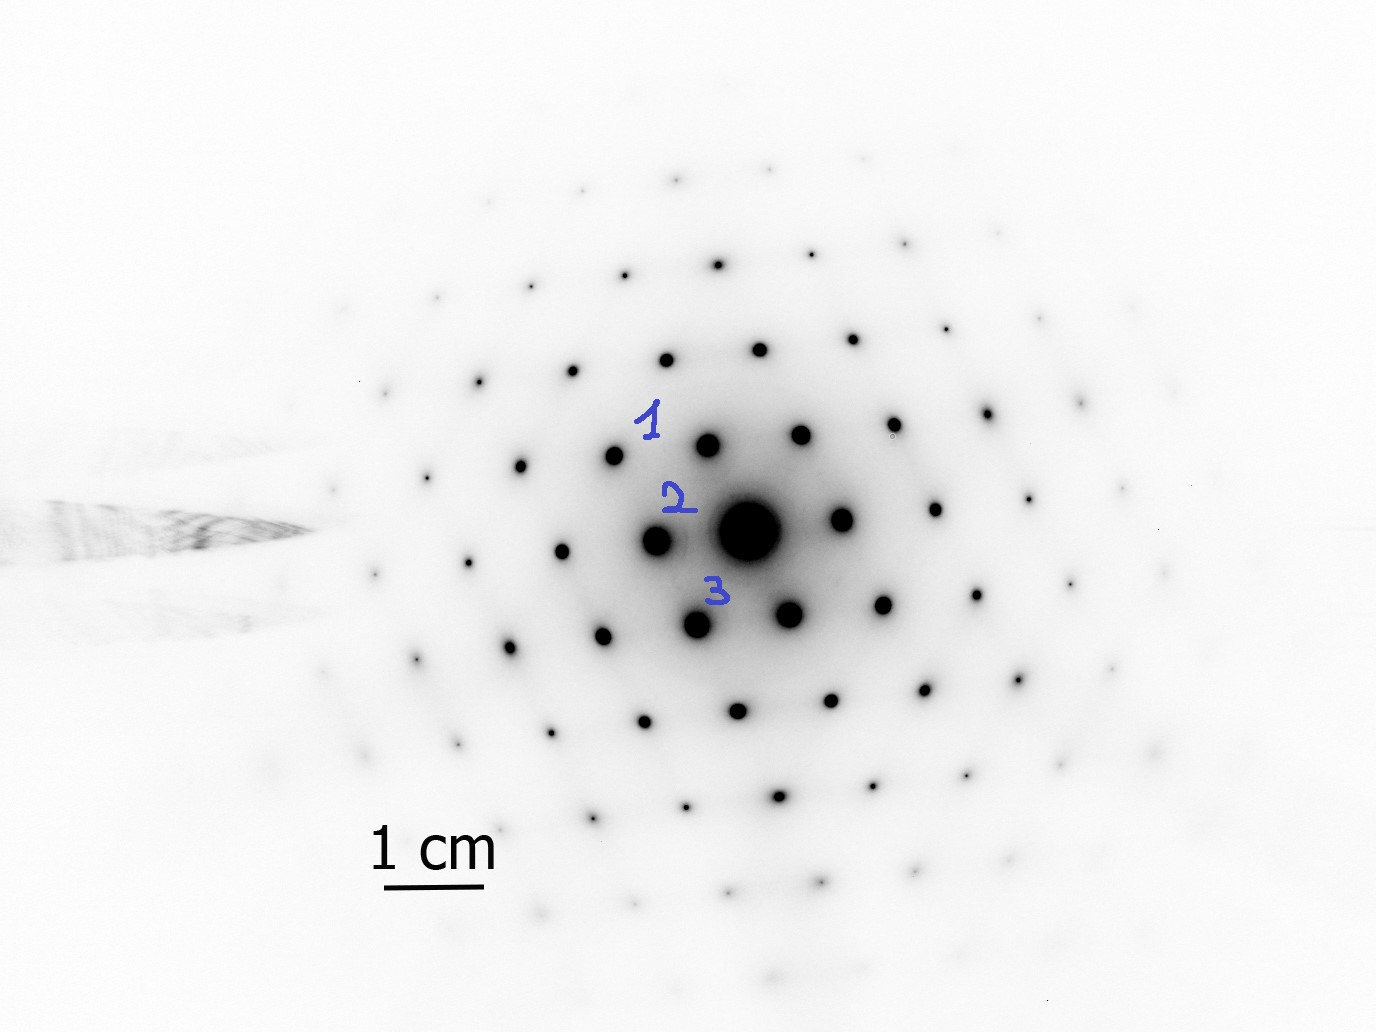
\includegraphics[width=0.7\linewidth, angle=90]{T2}
	\caption{Исследуемая кольцевая электронограмма}
	\label{fig:dots}
\end{figure}

Для получения из электронограммы интересующего нас межплоскостного расстояния предлагается воспользоваться формулой

\begin{equation}
	d = \frac{C}{2 R} = \frac{45}{2 R}
\end{equation}

Здесь $R$ --- радиус-вектор рефлекса, $C$ --- постоянная, определяемая характеристиками прибора. В нашем случае подставляем $C = 45$, в таком случае получаем $d$ в ангстремах при условии, что $R$ подставляем в миллиметрах. Результат измерения $d$ можно увидеть в таблице.

Кроме того, проиндексируем три рефлекса, выделенные на электронограмме. Положим, что центральный рефлекс имеет индексы (000), тогда для индексации остальных нам необходимо определить углы между направлениями на них. Для этого воспользуемся теоремой косинусов и уже определенными нами радиус-векторами. Полученные углы сопоставим тем, которые приведены в имеющейся таблице для определения индексов рефлексов, из которой подходящими оказались следующие: %чуто

В качестве дополнительной проверки отметим, что визуально электронограмма похожа на картину, получаемую от проекции ГЦК в направлении [110] (см. рисунок )% рисунок с гцк
При этом индексы, определенные нами, в точности совпадают с приведенными на рисунке индексами, что также свидетельствует о корректности индексации.

Наконец, имея в наличии межплоскостные расстояния и индексы, а также понимая, что мы имеем дело с ГЦК, поиском по базе данных попытаемся определить материал. Вероятными кандидатами являются Al и Ag, и я скорее склоняюсь в сторону Al.


\section{Расчет кольцевой электронограммы}

Расчет был произведен для представленной на рисунке \ref{fig:circle} электронограммы. Промеренные радиусы колец приведены в сводной таблице, с учетом масштаба. После этого, согласно тому, что $d = 1 / R$, были получены межплоскостные расстояния $d$, указанные в той же таблице.

\begin{figure}[H]
	\centering
	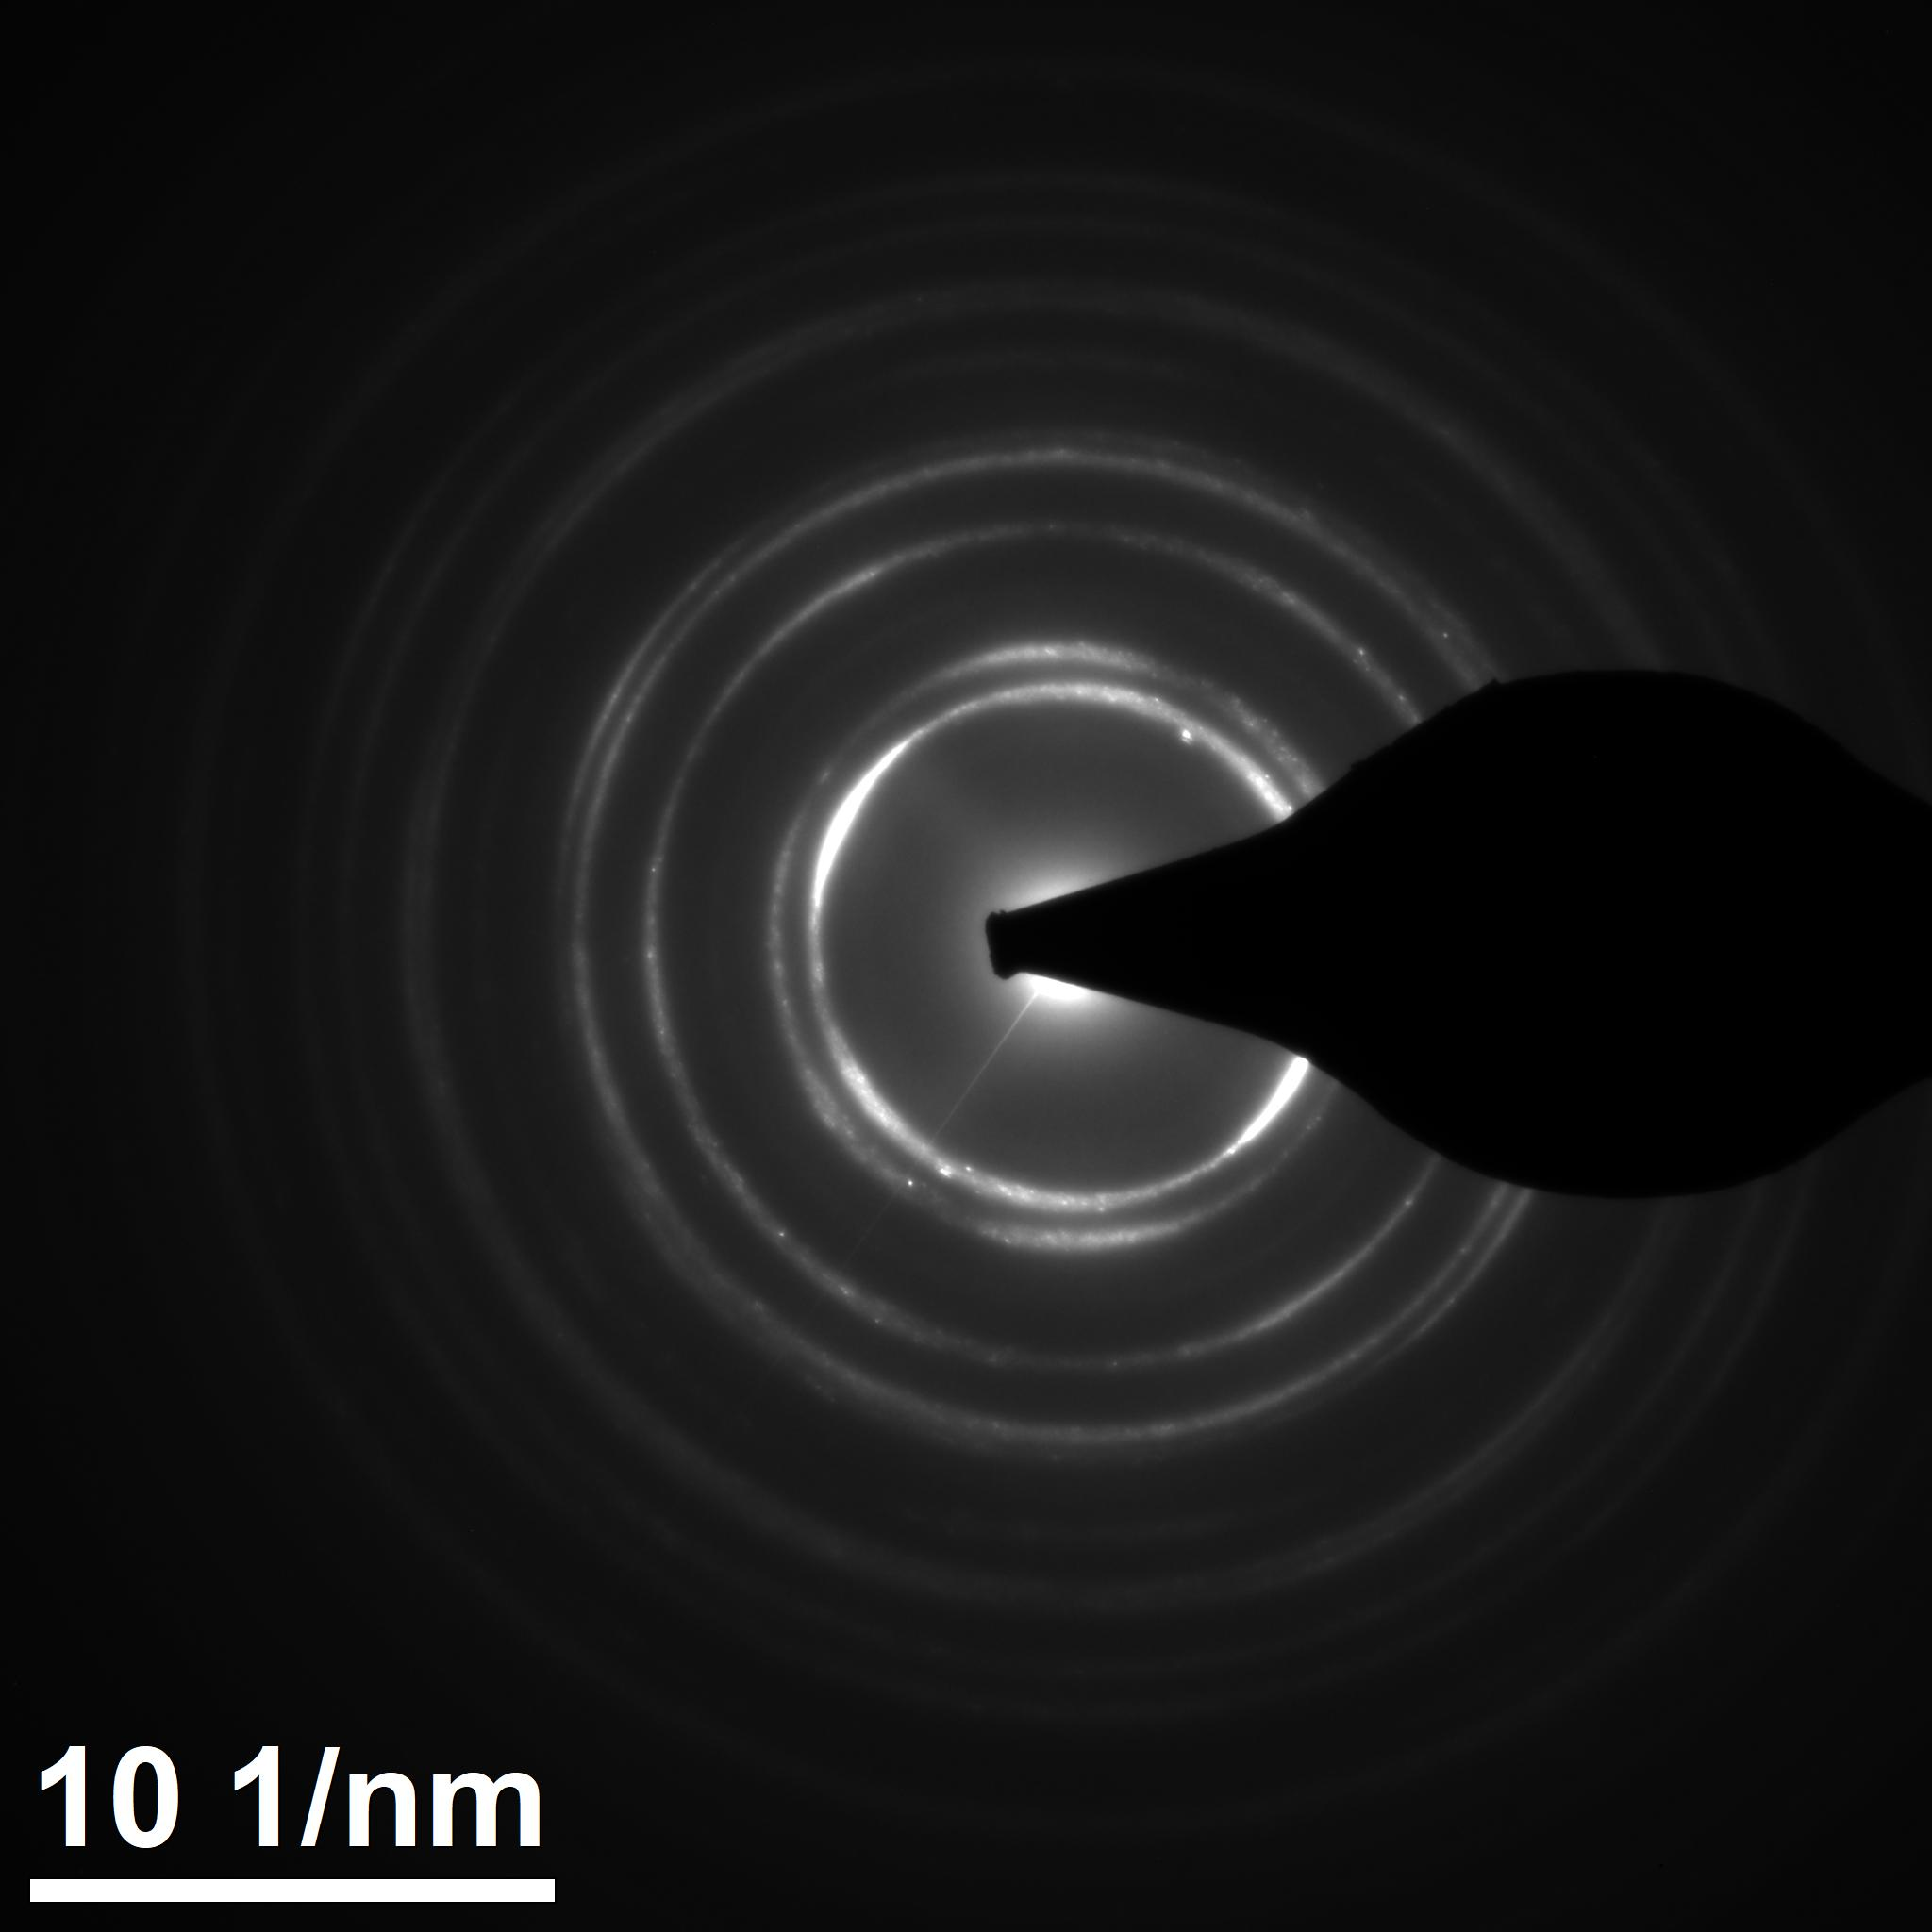
\includegraphics[width=0.7\linewidth]{K3} 
	\caption{Исследуемая кольцевая электронограмма}
	\label{fig:circle}
\end{figure}

С учетом того, что в разработке есть указание искать совпадение среди таких элементов как никель, железо алюминий, была проведена сверка полученных расстояний с имеющимися в программе Match! картотеками. По результату оказалось, что лучше всего подходит никель, его карточка для сравнения приведена на рисунке \ref{fig:Nikel}. Также из картотеки узнаем и интересующие нас параметр решетки ($a = 3.52$~\AA), а также тип кристаллической решетки --- кубическая гранецентрированная.

\begin{table}[H]
	\centering
	\begin{tabular}{|c|c|c|}
		\hline
		N & R, 1/nm & d, nm \\
		\hline
		1 & 4.93 & 0.203  \\
		\hline
		2 & 5.76 & 0.173  \\
		\hline
		3 & 8.11 & 0.123  \\
		\hline
		4 & 9.56 & 0.105  \\
		\hline
		5 & 9.99 & 0.100  \\
		\hline
		6 & 11.32 & 0.088 \\
		\hline
		7 & 12.55 & 0.080  \\
		\hline
		8 & 12.90 & 0.078  \\
		\hline
	\end{tabular}
\end{table}

\begin{figure}[H]
	\centering
	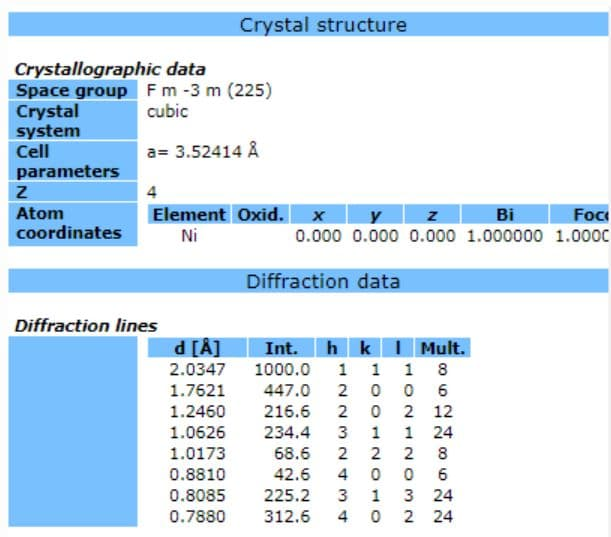
\includegraphics[width=0.5\linewidth]{Nikel}
	\caption{Карточка никеля из картотеки Match!}
	\label{fig:Nikel}
\end{figure}


\newpage

\begin{thebibliography}{1}
	\bibitem{Practicum}
	Рентгендифракционные методы изучения структуры монокристаллов, поликристаллических и аморфных материалов
\end{thebibliography}


\end{document}